%******************************************************************************%
%                                                                              %
%                                 Interlude                                    %
%                         for Machine Learning module                          %
%                                                                              %
%******************************************************************************%

% =============================== %
\section*{Interlude - Evaluate}
% ------------------------------- %

\begin{figure}[!h]
    \centering
    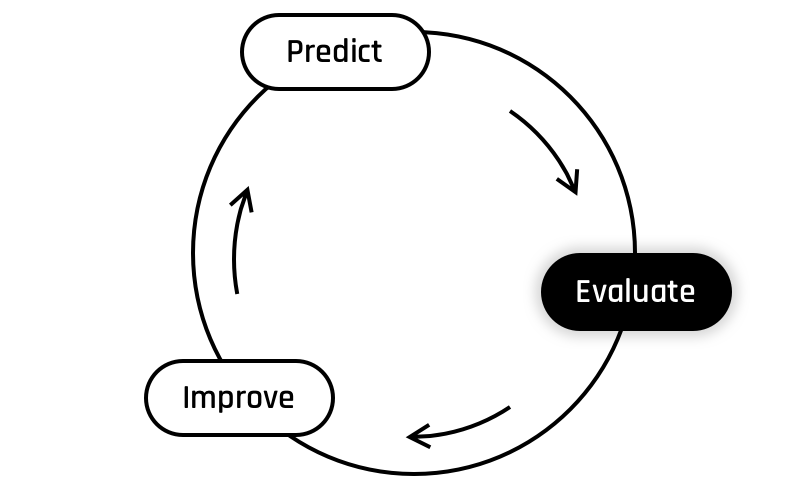
\includegraphics[scale=0.25]{assets/Evaluate.png}
    %\caption{The Learning Cycle: Evaluate}
\end{figure}


% =============================== %
\section*{Back to the Loss Function}
% ------------------------------- %
How is our model doing?  

To evaluate our model, remember before we used a \textbf{metric} called the \textbf{loss function} (also known as \textbf{cost function}).
The loss function is basically just a measure of how wrong the model is, in all of its predictions.

Two modules ago, we defined the loss function as the average of the squared distances between each prediction and its expected value (distances represented by the dotted lines in the figure below):

\begin{figure}[!h]
    \centering
    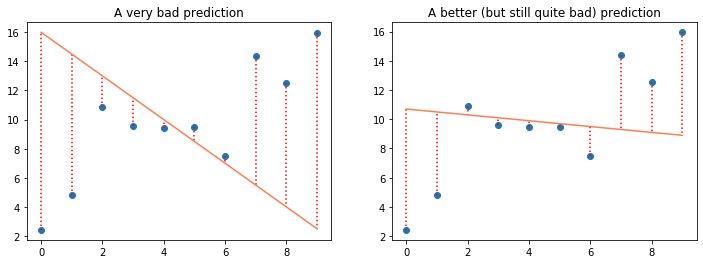
\includegraphics[scale=0.5]{assets/bad_pred_with_distance.png}
    \caption{Distances between predicted and expected values}
\end{figure}

The formula was the following: 

$$
J(\theta) = \frac{1}{2m}\sum_{i=1}^{m}(\hat{y}^{(i)} - y^{(i)})^2
$$

And its vectorized form:

$$
\begin{matrix}
J(\theta) = \frac{1}{2m}(\hat{y} - y)\cdot(\hat{y}- y)
\end{matrix}
$$  

\textit{So, now that we moved to multivariate linear regression, what needs to change?}\newline
You may have noticed that variables such as $x_j$ and $\theta_j$ don't intervened in the equation.
Indeed, the loss function only uses the predictions ($\hat{y}$) and the expected values ($y$), so the inner workings of the model don't matter to its evaluation metric.

This means we can use the exact same loss function as we did before!
